\newpage

\section{Pengujian dan analisis}
Pada bab ini, akan dijelaskan mengenai hasil pengujian dan pembahasan dari penelitian yang telah diuraikan pada metodologi. Selain itu, akan dipaparkan juga mengenai skenario pengujian yang dilakukan untuk mengevaluasi performa sistem secara keseluruhan. Pengujian ini dilakukan dengan tujuan untuk memastikan bahwa sistem yang dirancang mampu berfungsi dengan baik dalam memprediksi apakah pelanggan akan churn atau tidak berdasarkan data yang telah diproses pada tahap sebelumnya.


\subsection{Pengujian Sistem}
Pengujian sistem dilakukan dengan menggunakan dataset yang telah diolah sebelumnya dan dibagi menjadi data latih dan data uji. Data latih digunakan untuk melatih model Logistic Regression, sedangkan data uji digunakan untuk menguji performa model yang telah dilatih. Adapun skenario pengujian yang dilakukan adalah sebagai berikut:
\begin{enumerate}
    \item \textbf{Pengujian Model Logistic Regression:} Model Logistic Regression dilatih menggunakan data latih yang telah disiapkan. Proses pelatihan ini melibatkan penyesuaian parameter model untuk memaksimalkan akurasi prediksi terhadap data latih.
    \item \textbf{Perbandingan dengan Model Lain:} Jika ada, model lain yang lebih kompleks seperti Decision Tree, Random Forest atau XGBoost juga diuji untuk membandingkan performa dengan model Logistic Regression. Hal ini dilakukan untuk melihat apakah model yang lebih kompleks memberikan hasil yang lebih baik dalam memprediksi churn pelanggan.
\end{enumerate}

\subsection{Pengujian model Logistic Regression}
Pengujian model Logistic Regression dilakukan dengan menggunakan data uji yang telah disiapkan. Model ini dilatih pada data latih dan kemudian diuji pada data uji untuk mengevaluasi performanya. Hasil dari pengujian ini akan memberikan gambaran tentang seberapa baik model dalam memprediksi churn pelanggan.

Setelah dilakukan pengujian model Logistic Regression, diperoleh hasil confusion matrix yang merepresentasikan performa model dalam mengklasifikasikan data uji. Confusion matrix ini menunjukkan jumlah prediksi yang benar dan salah untuk masing-masing kelas (churn dan tidak churn). Dari confusion matrix, dapat dihitung beberapa metrik evaluasi seperti akurasi, presisi, recall, dan F1-score.

\newpage
\subsubsection{Hasil Logistic Regression tanpa hyperparameter tuning}

Berikut adalah hasil confusion matrix dari model Logistic Regression yang telah diuji pada data uji, Gambar \ref{fig:confusion_matrix_logistic_regression} menunjukkan confusion matrix yang diperoleh dari model Logistic Regression tanpa melakukan hyperparameter tuning.

\begin{figure}[H]
    \centering
    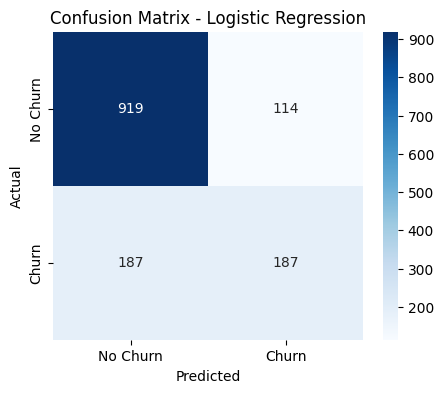
\includegraphics[width=0.4\textwidth]{gambar/logisticregression.png}
    \caption{Confusion Matrix Model Logistic Regression}
    \label{fig:confusion_matrix_logistic_regression}
\end{figure}

Dari gambar \ref{fig:confusion_matrix_logistic_regression} kita bisa identifikasi performa model Logistic Regression dalam mengklasifikasikan data uji. Confusion matrix ini memberikan informasi tentang jumlah prediksi yang benar dan salah untuk masing-masing kelas (churn dan tidak churn). Detailnya adalah sebagai berikut:

% True Negative (TN) = 919
% (Pelanggan yang benar-benar tidak churn dan diprediksi tidak churn)

% False Positive (FP) = 114
% (Pelanggan yang tidak churn, tetapi diprediksi churn)

% False Negative (FN) = 187
% (Pelanggan yang churn, tetapi diprediksi tidak churn)

% True Positive (TP) = 187
% (Pelanggan yang benar-benar churn dan diprediksi churn)

\begin{itemize}
    \item True Negative (TN): 919 (Pelanggan yang benar-benar tidak churn dan diprediksi tidak churn)
    \item False Positive (FP): 114 (Pelanggan yang tidak churn, tetapi diprediksi churn)
    \item False Negative (FN): 187 (Pelanggan yang churn, tetapi diprediksi tidak churn)
    \item True Positive (TP): 187 (Pelanggan yang benar-benar churn dan diprediksi churn)
\end{itemize}

% masukan semua hasil prediksi kedalam rumus pencarian accuracy, recall, precision
Setelah mendapatkan confusion matrix, kita dapat menghitung beberapa metrik evaluasi untuk model Logistic Regression. Metrik yang umum digunakan adalah akurasi, presisi, recall, dan F1-score. 

Akurasi adalah proporsi prediksi yang benar dari total prediksi yang dilakukan oleh model. Berikut adalah perhitungan akurasi model Logistic Regression:
\begin{equation}
    \text{Akurasi} = \frac{TP + TN}{TP + TN + FP + FN} = \frac{187 + 919}{187 + 919 + 114 + 187} = \frac{1106}{1407} \approx 0.785
\end{equation}

Presisi adalah proporsi prediksi positif yang benar dari total prediksi positif yang dilakukan oleh model. Berikut adalah perhitungan presisi model Logistic Regression:

\begin{equation}
\text{Presisi} = \frac{TP}{TP + FP} = \frac{187}{187 + 114} = \frac{187}{301} \approx 0.621
\end{equation}
    
Recall adalah proporsi prediksi positif yang benar dari total kasus positif yang sebenarnya. Berikut adalah perhitungan recall model Logistic Regression:

\begin{equation}
\text{Recall} = \frac{TP}{TP + FN} = \frac{187}{187 + 187} = \frac{187}{374} \approx 0.500
\end{equation}
    
F1-score adalah rata-rata harmonis dari presisi dan recall, yang memberikan gambaran keseluruhan tentang performa model. Berikut adalah perhitungan F1-score model Logistic Regression:

\begin{equation}
F1\text{-score} = 2 * \frac{\text{Presisi} * \text{Recall}}{\text{Presisi} + \text{Recall}} = 2 * \frac{0.621 * 0.500}{0.621 + 0.500} = 2 * \frac{0.3105}{1.121} \approx 0.553
\end{equation}

%Interpretasi hasilnya
Hasil evaluasi model Logistic Regression menunjukkan bahwa model ini memiliki akurasi sekitar 78.5\%, presisi sekitar 62.1\%, recall sekitar 50.0\%, dan F1-score sekitar 55.3\%. Meskipun akurasi model cukup baik, namun nilai recall yang rendah menunjukkan bahwa model ini cenderung kesulitan dalam mengidentifikasi pelanggan yang benar-benar churn. Hal ini dapat menjadi perhatian bagi perusahaan, karena kehilangan pelanggan yang churn dapat berdampak signifikan terhadap pendapatan.

Selain confusion matrix didapatkan juga nilai ROC-AUC yang merupakan metrik evaluasi yang umum digunakan untuk model klasifikasi. Nilai ROC-AUC berkisar antara 0 hingga 1, di mana nilai 1 menunjukkan model yang sempurna dan nilai 0.5 menunjukkan model yang tidak lebih baik dari tebakan acak. Nilai ROC-AUC yang diperoleh dari model Logistic Regression adalah sekitar 0.8286 yang menunjukkan bahwa model ini memiliki kemampuan yang baik dalam memisahkan kelas churn dan tidak churn. Nilai ini menunjukkan bahwa model Logistic Regression dapat digunakan sebagai dasar untuk prediksi churn pelanggan, meskipun masih ada ruang untuk perbaikan.